\newcommand{\lecturetitle}[1]{
  \title{01204211 Discrete Mathematics \\ #1}
  \author{Jittat Fakcharoenphol}
  \frame{\titlepage}
}
\newcommand{\Mod}{\,\bmod\,}


\newcommand\sbullet[1][.5]{\mathbin{\vcenter{\hbox{\scalebox{#1}{$\bullet$}}}}}

\lecturetitle{Lecture 12b: Undecidability (2)}
\renewcommand{\epsilon}{\varepsilon}

\newcommand{\czero}{{\mathtt 0}}
\newcommand{\cone}{{\mathtt 1}}
\newcommand{\sigcupgam}{\Sigma\cup\Gamma}


\frame{
  \frametitle{Decision problems}

  \begin{itemize}
  \item Given an integer $x$, is $x$ odd?
  \item Given a string $w$, is $w$ palindrome?
  \item Given a string $w$, is $w\in\{\czero^n\cone^n\;|\;n\geq 0\}$?
  \item Given a map, a starting position $s$, a destination $t$, and
    an integer $k$, does there exist a path from $s$ to $t$ with
    distance at most $k$?
  \item Given a program $P$ and input string $w$, when running $P$
    with $w$ as an input, does $P$ terminate?
  \end{itemize}
}

\frame{
  \frametitle{Decision problems and languages}

  For this problem:
  
  \begin{block}{}
    Given an integer $x$, is $x$ odd?
  \end{block}

  we can define a corresponding language
  \[
  L_E=\{,\ldots,-6,-4,-2,0,2,4,6,\ldots\}.
  \]

  To solve this problem, given $x$, we can ask if $x\in L_E$.
  
}

\frame{
  \frametitle{Deciders}

  We say that a python program $P$ {\color{red}\bf decides} the
  language $L$ if for any input string $x$, $P$ when running with $x$
  as an input,
  \begin{itemize}
  \item $P$ always terminates, 
  \item $P$ outputs {\tt\bf yes}, if $x\in L$, and
  \item $P$ outputs {\tt\bf no}, if $x\not\in L$.
  \end{itemize}

  \pause  

  If we believe that anything that a computer can do can be written as
  a python program, and there is no python program that decides a
  language $A$, then we say that

  \begin{block}{}
    $A$ is undecidable.
  \end{block}
}

\frame{
  \frametitle{Language {\sc HaltA} and {\sc Halt}}

  Let ${\mathbb P}$ be the set of all python programs.  Let the
  language {\sc HaltA} be
  \[
  \{ P\in {\mathbb P} \;|\; \mbox{when running $P$ with $P$ as an
    input, $P$ terminates} \}
  \]
  
  Or with a more concise notation:
  \[
  \textsc{HaltA} = \{ P\in {\mathbb P} \;|\; \mbox{$P(P)$ terminates} \}.
  \]

  We also have another related language
  \[
  \textsc{Halt} = \{ (P,w) \;|\;
  \mbox{$P$ is a python program such that $P(w)$ terminates}
  \}
  \]

}

\begin{frame}
  \begin{lemma}
    {\sc HaltA} and {\sc Halt} are undecidable.
  \end{lemma}
\end{frame}

\begin{frame}[fragile=true]

  \begin{lemma}
    There is no python program that decides $A$.
  \end{lemma}
  \begin{proof}
    We prove by contradiction. Assume that there is a python program
    $P$ that decides $A$.  \pause

    We describe a python program $B$ that reads a string $Q$ as an
    input as follows:

    {\small
\begin{verbatim}
Program B
Input Q
1.    Load P as module Pmod
2.    if Pmod.main(Q) == 'yes':    # when Pmod outputs yes
3.       while True: pass          #   loop forever 
4.    else:                        # when Pmod outputs no
5.       quit()                    #   halt
\end{verbatim}
    }

    Given program $Q$ as an input, $B$ loops forever when \pause

    It terminates when
  \end{proof}
\end{frame}

\frame{
  \begin{proof}
    We know that
    \begin{itemize}
    \item $B(Q)$ loops when $Q(Q)$ terminates, and
    \item $B(Q)$ terminates when $Q(Q)$ loops.
    \end{itemize}

    Does running $B$ using $B$ as an input terminate?

    \pause

    Let's try to plug in $Q=B$.  We have
    \begin{itemize}
    \item $B(B)$ loops when \pause $B(B)$ terminates, \pause and
    \item $B(B)$ terminates when \pause $B(B)$ loops. \pause
    \end{itemize}

    Since either $B(B)$ loops or terminates, and we cannot be in any
    of the cases, we obtain a contradiction.

    Therefore, we conclude that program $P$ does not exist.
  \end{proof}
}

\begin{frame}
  \frametitle{Reduction: proving undecidability of {\sc Halt}}

  \begin{itemize}
  \item We show that if {\sc Halt} is decidable, then {\sc HaltA} is
    also decidable.
  \item However, {\sc HaltA is undecidable}.
  \item We conclude that {\sc Halt} is also undecidable.
  \end{itemize}
\end{frame}

\frame{
  \frametitle{Reduction in picture}
}

\begin{frame}[fragile=true]
  
  {\small
    Let $\textsc{Accept} = \{(P,w) \;|\;
    \mbox{$P\in{\mathbb P}$ and $P(w)$ terminates with acceptance}\}.$
  }
  
  \begin{lemma}
    {\sc Accept} is undecidable.
  \end{lemma}
  \begin{block}{Proof.}

      We prove the lemma by contradiction.  Assume that there is a
      python program $Q$ that decides {\sc Accept}.  We
      construct a program $C$ that decides {\sc Halt} as follows 
      
      {\footnotesize
\begin{verbatim}
Program C       
Input P,w       
1.   Replace every "print('no')" statement in P with "print('yes')"
1.   if Q(P,w) == 'yes':
2.      print('yes')
3.   else
4.      print('no')
\end{verbatim}
      }

  \end{block}
\end{frame}

\begin{frame}[fragile=true]
  \begin{proof}[Proof (cont.)]
    {\footnotesize
\begin{verbatim}
Program C       
Input P,w       
1.   Replace every "print('no')" statement in P with "print('yes')"
1.   if Q(P,w) == 'yes':
2.      print('yes')
3.   else
4.      print('no')
\end{verbatim}
    }   
    {\small
      We have to make sure that our reduction is correct by considering
      two cases.
      
      Case 1: when $P(w)$ halts. \pause

      Case 2: when $P(w)$ does not halt. \pause

      Since in both cases, $C$ answers correctly, we know that given
      program $Q$ deciding {\sc Accept}, we can construct a program
      $C$ that decides {\sc Halt}.  However, we know that {\sc Halt}
      is undecidable; thus, we reach a contradiction.  We conclude
      that {\sc Accept} is also undecidable.  }
  \end{proof}
\end{frame}

\frame{
  \frametitle{Reduction from {\sc Halt} to {\sc Accept} in picture}
  
}

\frame{
  \frametitle{How about {\sc Reject}?}

  Let
  \[
  \textsc{Reject} = \{(P,w) \;|\;
  \mbox{$P\in{\mathbb P}$ and $P$ rejects $w$}\}.
  \]

  
}
\frame{
  \frametitle{How about {\sc NotHalt}?}

  Let
  \[
  \textsc{NotHalt} = \{(P,w) \;|\;
  \mbox{$P\in{\mathbb P}$ and $P(w)$ does not terminate}\}.
  \]

  
}

\frame{
  \frametitle{Language of program $P$}

  For a python program $P$, let $L(P)$ be the set of all strings that
  $P$ accepts, i.e.,

  \[
  L(P) = \{ w\in\Sigma^* \;|\; P(w)=yes \}.
  \]

  Let
  \[
  \textsc{All} =
  \{
  P\in{\mathbb P} \;|\; L(P)=\Sigma^*
  \}.
  \]

}

\begin{frame}[fragile=true]
  \begin{lemma}
    {\sc All} is undecidable.
  \end{lemma}
  \begin{block}{Proof.}
    {\small
      
    We prove by reduction from {\sc Halt}.  Assume that {\sc All} is
    decidable, i.e., there is a python program $Q$ that decides {\sc
      All}.  We construct program $C$ that decides {\sc Halt} as
    follows

    {\footnotesize
\begin{verbatim}
Program C (input: P,w)
1. Construct another program R from P and w:
     | Program R (input: x)
     | 1.  Run program P on input w, suppressing any output from P
     | 2.  Accept x
2. if Q(R) == 'yes':
3.     return 'yes'
4. else: return 'no'
\end{verbatim}
    }
    }
  \end{block}
\end{frame}

\begin{frame}[fragile=true]
  \begin{proof}[Proof (cont.)]
    {\footnotesize
\begin{verbatim}
Program C (input: P,w)
1. Construct another program R from P and w:
     | Program R (input: x)
     | 1.  Run program P on input w, suppressing any output from P
     | 2.  Accept x
2. if Q(R) == 'yes':
3.     return 'yes'
4. else: return 'no'
\end{verbatim}
    }
    {\small
      To ensure the correctness, we have to consider two cases.

      Case 1: when $P(w)$ halts. \pause
      
      Case 2: when $P(w)$ does not halt. \pause

      Since we can construct a program for {\sc Halt} using a program
      that decides {\sc All}, but {\sc Halt} is undecidable;
      therefore, we conclude that {\sc All} is undecidable.
    }
  \end{proof}
\end{frame}

\frame{
  \frametitle{\sc Empty}

  Let
  \[
  \textsc{Empty} =
  \{
  P\in{\mathbb P} \;|\; L(P)=\emptyset
  \}.
  \]

}

\begin{frame}[fragile=true]
  \begin{lemma}
    {\sc Empty} is undecidable.
  \end{lemma}
  \begin{proof}
    {\small
      
    We prove by reduction from {\sc Halt}.  Assume that {\sc Empty} is
    decidable, i.e., there is a python program $Q$ that decides {\sc
      Empty}.  We construct program $C$ that decides {\sc Halt} as
    follows

    {\footnotesize
\begin{verbatim}
Program C (input: P,w)
1. Construct another program R from P and w:
     | Program R (input: x)
     | 1.  Run program P on input w, suppressing any output from P
     | 2.  Accept x
2. if Q(R) == 'yes':
3.     return 'no'
4. else: return 'yes'
\end{verbatim}
    }

    Since we can construct a program for {\sc Halt} using a program
    that decides {\sc Empty}, but {\sc Halt} is undecidable;
    therefore, we conclude that {\sc Empty} is undecidable.
    }
  \end{proof}
\end{frame}

\begin{frame}[fragile=true]
  \begin{lemma}
    Let $\textsc{Eq} = \{(P_1,P_2) \;|\;
    \mbox{$P_1,P_2\in{\mathbb P}$ and $L(P_1)=L(P_2)$}\}$.
    {\sc Eq} is undecidable.
  \end{lemma}
  \begin{proof}
    {\small
      
    We prove by reduction from {\sc All}.  Assume that {\sc Eq} is
    decidable, i.e., there is a python program $Q$ that decides {\sc
      Eq}.  We construct program $C$ that decides {\sc All} as
    follows

    {\footnotesize
\begin{verbatim}
Program C (input: P)
1. Construct another program R:
     | Program R (input: x)
     | 1.  Accept x
2. if Q(P,R) == 'yes':
3.     return 'yes'
4. else: return 'no'
\end{verbatim}
    }

    Since we can construct a program for {\sc All} using a program
    that decides {\sc Eq}, but {\sc All} is undecidable;
    therefore, we conclude that {\sc Eq} is undecidable.
    }
  \end{proof}
\end{frame}


\begin{frame}[fragile=true]
  \frametitle{Another proof for {\sc Eq}}
  
  \begin{proof}
    {\small
      
    We prove by reduction from {\sc Empty}.  Assume that {\sc Eq} is
    decidable, i.e., there is a python program $Q$ that decides {\sc
      Eq}.  We construct program $C$ that decides {\sc Empty} as follows

    {\footnotesize
\begin{verbatim}
Program C (input: P)
1. Construct another program R:
     | Program R (input: x)
     | 1.  Reject x
2. if Q(P,R) == 'yes':
3.     return 'yes'
4. else: return 'no'
\end{verbatim}
    }

    Since we can construct a program for {\sc Empty} using a program
    that decides {\sc Eq}, but {\sc Empty} is undecidable; therefore,
    we conclude that {\sc Eq} is undecidable.
    }
  \end{proof}
\end{frame}

\begin{frame}[fragile=true]
  \begin{lemma}
    Let $\textsc{Hello} = \{ P\in{\mathbb P} \;|\;
    L(P)=\{\texttt{hello}\}\}$.
    {\sc Hello} is undecidable.
  \end{lemma}
  \begin{proof}[INCORRECT PROOF]
      We prove by reduction from {\sc Eq}.  Assume that {\sc Eq} is
      decidable, i.e., there is a python program $Q$ that decides {\sc
        Eq}.  We construct program $C$ that decides {\sc Hello} as
      follows

      {\footnotesize
\begin{verbatim}
Program C (input: P)
1. Construct another program R:
     | Program R (input: x)
     | 1.  if x == 'hello':
     | 2.    print('yes')    # accept x
     | 3.  else
     | 4.    print('no')     # reject x
2. if Q(P,R) == 'yes':
3.     return 'yes'
4. else: return 'no'
\end{verbatim}
      }
  \end{proof}
\end{frame}

\begin{frame}[fragile=true]
  \begin{lemma}
    Let $\textsc{Hello} = \{ P\in{\mathbb P} \;|\;
    L(P)=\{\texttt{hello}\}\}$.
    {\sc Hello} is undecidable.
  \end{lemma}
  \begin{block}{Proof}
      We prove by reduction from {\sc Halt}.  Assume that {\sc Hello}
      is decidable, i.e., there is a python program $Q$ that decides
      {\sc Hello}.  We construct program $C$ that decides {\sc Halt}
      as follows

      {\footnotesize
\begin{verbatim}
Program C (input: P,w)
1. Construct another program R:
     | Program R (input: x)
     | 1.  if x != 'hello':
     | 2.    print('no')     # reject x
     | 3.  Replace any output statements from P
     | 4.  Run the modified P on w 
     | 5.  print('yes')      # accept x
2. if Q(R) == 'yes':
3.     return 'yes'
4. else: return 'no'
\end{verbatim}
      }
  \end{block}
\end{frame}


\begin{frame}[fragile=true]
  \begin{proof}[Proof (cont.)]
    {\tiny
\begin{verbatim}
Program C (input: P,w)
1. Construct another program R:
     | Program R (input: x)
     | 1.  if x != 'hello':
     | 2.    print('no')     # reject x
     | 3.  Replace any output statements from P
     | 4.  Run the modified P on w 
     | 5.  print('yes')      # accept x
2. if Q(R) == 'yes':
3.     return 'yes'
4. else: return 'no'
\end{verbatim}
    }
    {\small
      We consider two cases:

      Case 1: $P(w)$ halts. \pause

      Case 2: $P(w)$ does not halt. \pause

      Since we can construct a program that decides {\sc Halt} given a
      program that decides {\sc Hello}, but {\sc Halt} is undecidable.
      We conclude that {\sc Hello} is also undecidable.
    }
  \end{proof}
\end{frame}

\frame{
  \frametitle{Python as computation}

  Do you believe in this assumption:

  {\bf Anything that a computer can do can be written as a python
    program. }

}

\frame{
  \frametitle{Turing machines}

  {\bf Anything that a computer can do can be carried out using Turing
    machines. }

  \vspace{0.3in}
  \pause
  
  {\bf Any possible computation can be performed by Turing machines. }

}

\frame{
  \frametitle{Turing Machines}

  \pause
  
  \begin{itemize}
  \item Proposed by Alan Turing in 1936.
    \pause
  \item A finite automaton with an \structure{unlimited} memory with
    \structure{unrestricted} access.  
    \pause
  \item Can perform any tasks that a computer can.  (we'll see)
    \pause
  \item However, there are problems that TM can't solve.  These
    problems are beyond the limit of computation.
  \end{itemize}
}

\frame{
  \frametitle{Components}

  \begin{itemize}
  \item An infinite \alert{\bf tape}.
  \item A tape head that can 
    \begin{itemize}
    \item \alert{\bf read and write} to the tape, and
    \item \alert{\bf move} around the tape.
    \end{itemize}
  \end{itemize}
}

\frame{
  \frametitle{Schematic}

  \begin{center}
    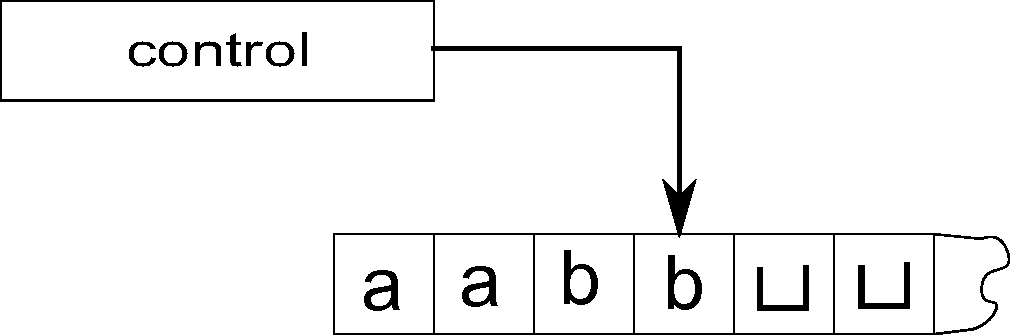
\includegraphics[scale=0.4]{images/tm.pdf}
  \end{center}
}

\frame{
  \frametitle{How Turing machines work}

  \begin{itemize}
  \item The tape initialy contains an input string.
    \pause
  \item The rest of the tape is blank (denoted by $\sqcup$).
    \pause
  \item The machine reads a symbol from of the tape where its head is
    at.
    \pause
  \item It can write a symbol back and move \alert{left} or
    \alert{right}.
    \pause
  \item At the end of the computation, the machine outputs
    \structure{accept} or \structure{reject}, by entering accept state
    of reject state.  (After changing, it halts.)
    \pause
  \item It can go on forever (not entering any accept or reject
    states).
  \end{itemize}
}

\begin{frame}
  \frametitle{Examples}
\end{frame}

\frame{
  \frametitle{Formal definition of a Turing Machine}

  \begin{itemize} 
  \item Again, the important part is the definition of
    the transition function.
    \pause
  \item The machine look at the tape \alert{symbol} and consider its
    \alert{current state}, then makes a move by \alert{writing some symbol}
    on the tape and \alert{moving its head left or right}.  \pause
  \item Thus,
    \begin{itemize}
    \item {\bf Input:} current state and the symbol on the tape \pause
    \item {\bf Output:} next state, a symbol to be written to the
      tape, and the new state. \pause
    \end{itemize}
    \pause
  \item So, $\delta$ is in the form: $Q\times\Gamma\to
    Q\times\Gamma\times\{\mathtt{LEFT},\mathtt{RIGHT}\}$ \pause
  \item E.g., if $\delta(q,a)=(r,b,\mathtt{LEFT})$, then if the machine is in
    state $q$ and reads $a$, it will change its state to $r$, write
    $b$ to the tape and move to the left.
  \end{itemize}

}

\frame{
  \frametitle{Definition}

  \begin{block}{Definition (Turing Machine)}
    A \alert{\bf Turing machine} is a 7-tuple,
    $(Q,\Sigma,\Gamma,\delta,q_0,q_{accept},q_{reject})$, where
    $Q,\Sigma,\Gamma$ are finite sets and
    \begin{enumerate}
    \item \alert{$Q$} is the set of states,
    \item \alert{$\Sigma$} is the input alphabet not containing the
      \alert{\bf blank symbol $\sqcup$},
    \item \alert{$\Gamma$} is the tape alphabet, where $\sqcup\in\Gamma$
      and $\Sigma\subset\Gamma$,
    \item $\delta: Q\times\Gamma\to Q\times\Gamma\times\{\mathtt{LEFT},\mathtt{RIGHT}\}$ is the transition function,
    \item $q_0\in Q$ is the start state,
    \item $q_{accept}\in Q$ is the accept state, and
    \item $q_{reject}\in Q$ is the reject state, where $q_{accept}\neq
      q_{reject}$.
    \end{enumerate}
  \end{block}
}

\frame{
  \frametitle{Variants of Turing Machines}
  \begin{itemize}
  \item There are many alternative definitions of TM's.
    \pause
  \item They are called \alert{variants} of TM's.
    \pause
  \item They all have the same power. This demonstrates the
    \alert{robustness} in the definition of TM's. \pause Also, this is
    an evidence that TM's ``capture'' the idea of computation (because
    whatever computing machine we can think of they are all equivalent
    to TM's).
  \end{itemize}
}

\frame{
  \frametitle{TM with ``stay put''}
  \begin{itemize}
  \item Let's start with an easy variant.  Suppose we allow additional
    head movement: ``stay put (S)''. \pause
  \item The transition function will be of the form
    \[
      \delta:Q\times\Gamma\to Q\times\Gamma\times\{\mathtt{LEFT},\mathtt{RIGHT},{\mathrm S}\}.
      \]
  \item Does this give TM's more power? \pause
  \item Not really.  We can convert a TM with ``stay put'' to a
    standard TM as follows. \pause
    \begin{itemize}
    \item For any ``stay put'' transition, we replace with two
      transitions: ``right'' and ``left''.
    \end{itemize}
  \end{itemize}

}

\frame{
  \frametitle{Multitape Turing Machines}
  \begin{itemize}
  \item A \alert{\bf multitape Turing machines} has many tapes.   \pause
  \item For each tape, the machine has a head for reading and writing
    it. \pause
  \item The input appears on tape 1; all other tapes contain blanks.
    \pause
  \item Let $k$ be the number of tapes.  The transition function can
    be defined as 
    \[
      \delta:Q\times\Gamma^k\to Q\times\Gamma^k\times\{\mathtt{LEFT},\mathtt{RIGHT},\mathtt{STAY}\}^k.
      \]
    \pause
  \item E.g., if $\delta(q_i,a_1,\ldots,a_k)=
    (q_j,b_1,\ldots,b_k,\mathtt{LEFT},\mathtt{RIGHT},\ldots,\mathtt{LEFT})$ then if the
    machine is at state $q_i$ and each head on tape $i$ reads symbol
    $a_i$, it'll write $b_i$ on each tape $i$, change state to $q_j$
    and move each head accordingly.
  \end{itemize}

}

\frame{
  \frametitle{Nondeterministic Turing Machines}
  \begin{itemize}
  \item A nondeterministic Turing machine can make
    ``nondeterministic'' move.  
    \pause
  \item As expected, its transition function has the form
    \[
      \delta:Q\times\Gamma\to{\mathcal P}(Q\times\Gamma\times\{\mathtt{LEFT},\mathtt{RIGHT}\}).
      \]
    \pause
  \item Again, we view the computation of a nondeterministic Turing
    machine as a tree, where each branching corresponds to the place
    where the TM can make different moves.
    \pause
  \item Can nondeterminism help?
  \end{itemize}
}

\frame{
  \frametitle{Equivalence in Power}

  \begin{itemize}
  \item {\bf Should I write programs in C or Pascal?}
    \pause
  \item {\bf Should I write programs in Python or Prolog?}
    \pause
  \item {\bf Should I write programs in Ruby or LISP?}
  \end{itemize}

}

\frame{
  \frametitle{They are all the same, in terms of computability}

  Since you can write a C interpreter in Pascal and Pascal interpreter
  in C, \pause what you can do in C, you can do in Pascal.

}

\frame{
  \frametitle{Turing machine}

  If you believe that Turing machines are ultimate model of computing,
  all those programming languages are equivalent because they all can
  simulate Turing machines (and they runs on Turing machines).

}

\frame{
  \frametitle{Two sides of a coin}

  \begin{itemize}
  \item Computers are powerful \pause (???) \pause
  \item How powerful? \pause
  \item To understand that, we want to see samples of tasks that
    computers \alert{can} do, and samples of tasks that they \alert{can't}
    do. \pause
  \item It's one story to show that computers can do something.  \pause
    It's another to show that computers can't do something.
    \begin{itemize}
    \item Maybe there's a limitation with ``this'' computer, but
      ``other'' computers might be able to do that thing.
    \item We want to be able to say that \alert{\bf for all} computers.
      \pause In fact, \alert{\bf for any ``thinkable''} computers.
    \end{itemize}
  \end{itemize}

}

\frame{
  \alert{\LARGE What is a computer?}
  \pause

  {\LARGE Something that computes?}
  \pause

  \alert{\LARGE What is computation?}
  \pause

  {\LARGE An act of following some instructions?}
  \pause

  {\LARGE An act of following some algorithm?}
  \pause

  \alert{\LARGE What is an algorithm?}
}

\frame{
  \frametitle{Hilbert's problems}

  Mathematician David Hilbert asked:

  {''Find a process according to which it can be determined by a
    finite number of operations if a given polynomial has intergral
    root''}

}

\frame{
  \frametitle{To say NO}

  We need an argument (a mathematical proof) that covers all possible
  ``processes'' or all ``computations''.

}

\frame{
  \frametitle{Possible definitions}

  \begin{itemize}
  \item Church's $\lambda$-calculus
  \item Turing's machines
  \end{itemize}
  \pause

  \alert{They both turned out to be {\bf equivalent}.}
}

\frame{

  \begin{block}{Church-Turing thesis}
    Turing machine algorithms = intuitive notion of algorithms
  \end{block}

}

\frame{
  \frametitle{Final answer to Hilbert}

  No, there doesn't exist any algorithm for determining if a
  polynomial has integral root.

}
